% !TEX root = ../../../main.tex
% 来源：中学数学实验教材·第二册（几何）
% 章节：实验几何 / 方向、角度与平行
% 原始文件：1.tex，行 1139-1150
% 类型：tikz
% ---
		\begin{tikzpicture}[>=latex, scale=1]
      \tkzDefPoints{0/0/B, 3/0/C, 1/2/A, 4/2/D,2/1/O}
\tkzDrawSegments(B,C A,B A,C C,D A,D B,D)
\tkzLabelPoints[below](B,C,O)	  
\tkzLabelPoints[above](A,D)	
\tkzMarkAngles[mark=none, size=.3](B,A,C A,O,B D,C,A)
\tkzMarkAngles[mark=none, size=.2](D,O,A)
\tkzLabelAngle[pos=.5](B,A,C){$\alpha$}
\tkzLabelAngle[pos=.5](A,O,B){$\gamma$}
\tkzLabelAngle[pos=.5](D,C,A){$\beta$}
\tkzLabelAngle[pos=.4](D,O,A){$\delta$}
		\end{tikzpicture}
